\footnotesize
\begin{tikzpicture}
\node at(-4,2){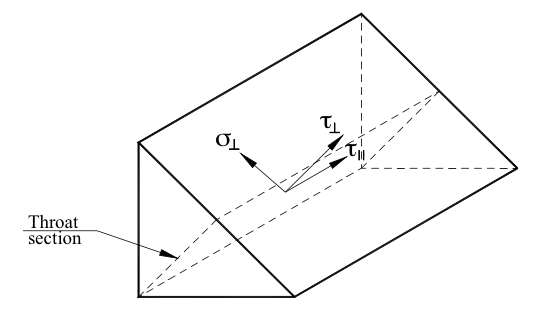
\includegraphics[width=6cm]{PIC/CH07/WSS}};
\draw(0,3)|-(3,0);
\draw[pattern=north east lines](2,0)--(0,2)|-cycle;
\draw(0,3)--++(20:5)coordinate(A)
(0,2)--++(20:5)coordinate(B)
(2,0)--++(20:5)coordinate(C)
(3,0)--++(20:5)coordinate(D);
\draw(A)--(B)--(C)--(D);
\dimline[extension start length=0,extension end length=0]{(0,-.5)}{(2,-.5)}{$t_w$};
\dimline[extension start length=0,extension end length=0]{(0,0)}{(1,1)}{$t_t$};
\dimline[extension start length=0,extension end length=0]{(3,0)}{($(3,0)+(20:5)$)}{$l_w$};
\end{tikzpicture}